\section{Task 4: Numerical Prediction}

The goal of this task is to predict a continuous numerical target using two regression algorithms. The target variable chosen is \texttt{stress}, which represents self-reported stress levels on a scale from 0 to 100. This variable was selected because it has the widest range and highest variance among all numeric columns in the dataset. It also shows the strongest correlations with other features, particularly sports hours ($r = -0.26$) and bedtime ($r = -0.23$). The other numeric candidates like \texttt{birth\_year} or \texttt{room\_estimate} have almost no correlation with any feature, making them poor regression targets.

\subsection*{Setup}

The cleaned dataset from Task 1B (\texttt{clean\_imputed\_simple.csv}) was used with 156 instances. Free-text columns (\texttt{good\_day\_1}, \texttt{good\_day\_2}) and the \texttt{random\_number} column were dropped. The random number column was removed because it contained extreme outlier values (up to $1.1 \times 10^{37}$) and carries no predictive signal for stress.

Categorical variables were preprocessed before modeling. The \texttt{programme} field was grouped to merge rare categories (fewer than 4 instances) into an "Other" label. Binary yes/no columns were encoded as 0/1, and the \texttt{stats\_course} column (which uses "mu" and "sigma" labels) was converted to a binary indicator. The timestamp was split into hour and weekday features. All numeric features were standardized, and the remaining categorical features were one-hot encoded.

The data was split into 80\% training (124 instances) and 20\% test (32 instances) using a fixed random seed of 42 for reproducibility.

\subsection*{Regression Approaches}

Two regression algorithms were compared:

\begin{itemize}
    \item \textbf{Ridge Regression}~\cite{hoerl_1970}: a linear model with L2 regularization. It penalizes large coefficients, which helps prevent overfitting on small datasets with many features after one-hot encoding.
    \item \textbf{Random Forest Regressor}~\cite{breiman_2001}: an ensemble of decision trees that captures non-linear relationships. Each tree is trained on a bootstrap sample, and the final prediction is the average across all trees.
\end{itemize}

Ridge was chosen as the linear baseline because standard linear regression tends to overfit when the number of features (after encoding) approaches the number of samples. Random Forest was chosen as the non-linear alternative because it handles mixed feature types well and does not assume a linear relationship between predictors and the target.

\subsection*{Hyperparameter Optimization}

Hyperparameters were tuned using grid search with 5-fold cross-validation on the training set, optimizing for negative mean squared error.

\begin{table}[h]
\caption{Hyperparameter search spaces and best configurations.}
\label{tab:task4_hyper}
\centering
\begin{tabular}{|l|l|l|}
\hline
Model & Search space & Best configuration \\
\hline
Ridge & alpha \{0.01, 0.1, 1.0, 10.0, 100.0\} & alpha = 100.0 \\
\hline
Random Forest & n\_estimators \{50, 100, 200\} & n\_estimators = 200 \\
 & max\_depth \{None, 5, 10, 15\} & max\_depth = 5 \\
 & min\_samples\_split \{2, 5, 10\} & min\_samples\_split = 10 \\
 & min\_samples\_leaf \{1, 2, 4\} & min\_samples\_leaf = 1 \\
\hline
\end{tabular}
\end{table}

The high alpha value selected for Ridge (100.0) indicates that strong regularization is needed. This makes sense given the small dataset and the relatively large number of features after one-hot encoding. For Random Forest, the shallow depth (5) and high split threshold (10) suggest the model also benefits from being constrained to avoid overfitting.

\subsection*{Results}

\begin{table}[h]
\caption{Task 4 regression performance for tuned models (target: \texttt{stress}).}
\label{tab:task4_results}
\centering
\begin{tabular}{|l|r|r|r|r|r|}
\hline
Model & CV RMSE & Test MSE & Test RMSE & Test MAE & Test $R^2$ \\
\hline
Ridge & 28.25 & 691.32 & 26.29 & 22.52 & 0.116 \\
Random Forest & 28.24 & 825.01 & 28.72 & 25.18 & $-$0.055 \\
\hline
\end{tabular}
\end{table}

Ridge outperforms Random Forest on the test set across all metrics. The test $R^2$ of 0.116 for Ridge is low but positive, meaning it explains about 12\% of the variance in stress levels. Random Forest achieves a negative $R^2$, which means it performs worse than simply predicting the mean stress value for every instance.

Both models had nearly identical cross-validation RMSE (around 28.2), but their test set behavior diverged. This gap is likely caused by the small test set size (32 samples), where a few difficult instances can shift the metrics noticeably.

\subsection*{Interpretation}

Figure~\ref{fig:task4_scatter} shows the actual versus predicted stress values for both models. Ridge predictions spread along a slight upward trend, indicating some ability to distinguish low-stress from high-stress students. Random Forest predictions cluster more tightly in the 30 to 60 range regardless of the actual value. This is a common pattern when a model defaults to predicting near the training set mean.

\begin{figure}[h]
\centering
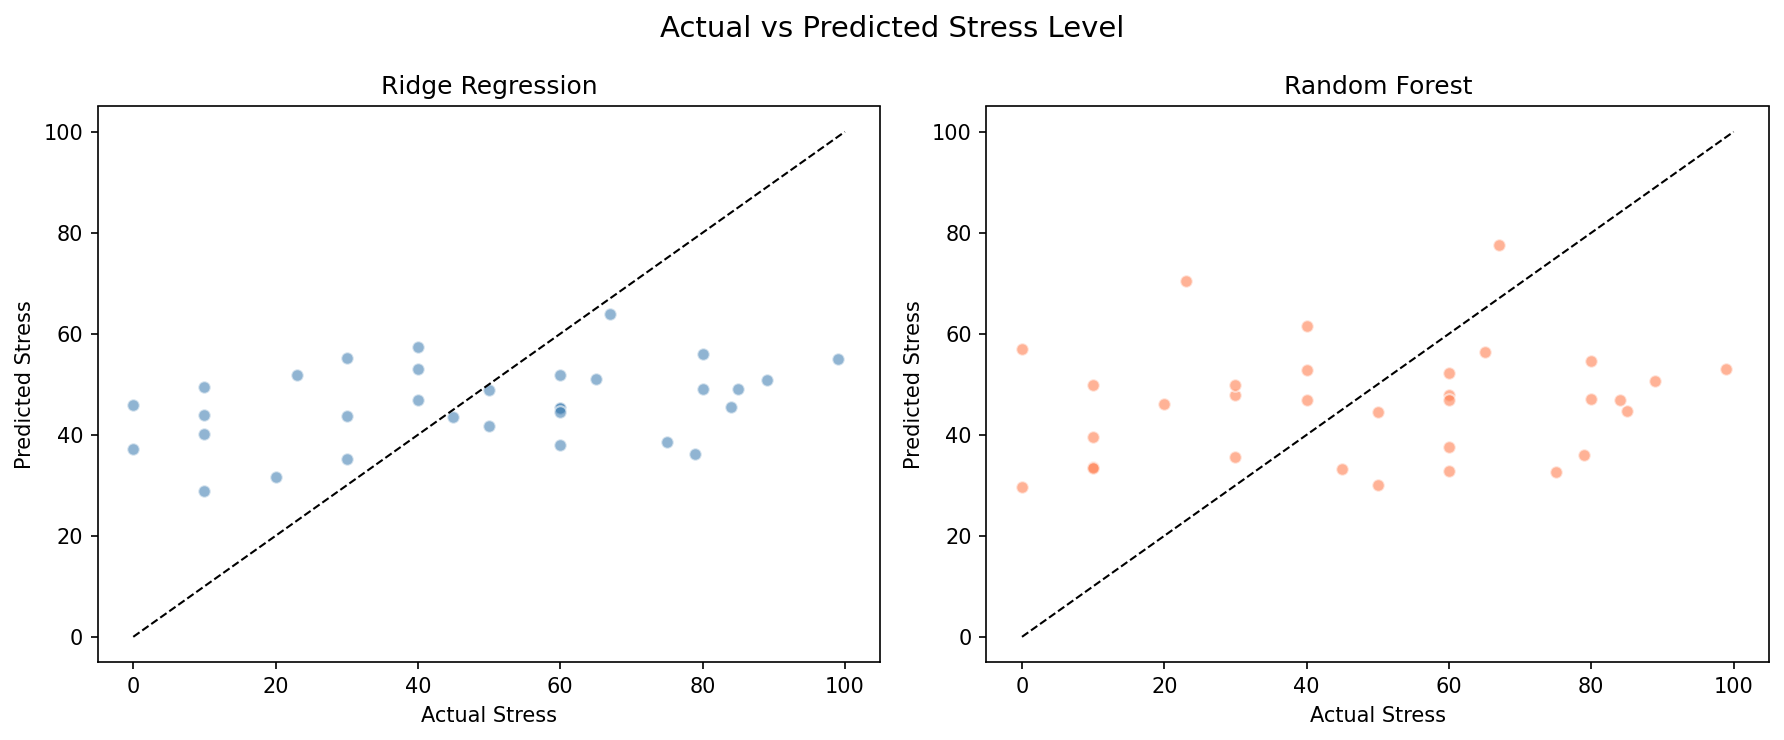
\includegraphics[width=\textwidth]{task4/task4_actual_vs_predicted.png}
\caption{Actual vs predicted stress levels for Ridge and Random Forest.}
\label{fig:task4_scatter}
\end{figure}

Figure~\ref{fig:task4_residuals} shows the distribution of residuals (actual minus predicted) for both models. Ridge residuals are spread roughly evenly around zero, while Random Forest residuals skew negative. The negative skew means the Random Forest tends to overpredict stress more often than it underpredicts it.

\begin{figure}[h]
\centering
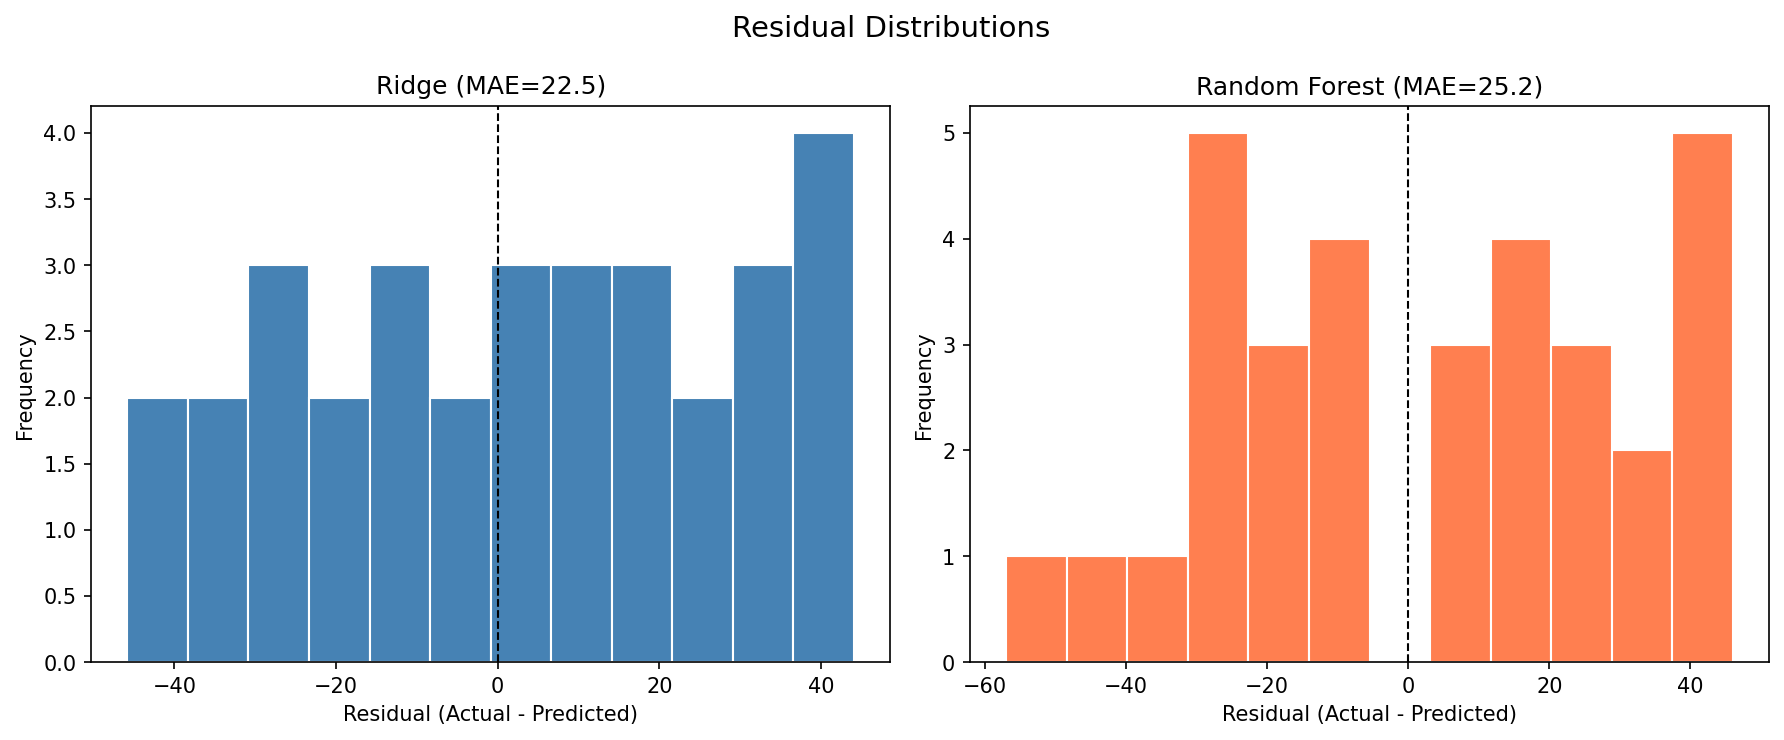
\includegraphics[width=\textwidth]{task4/task4_residuals.png}
\caption{Residual distributions for Ridge and Random Forest.}
\label{fig:task4_residuals}
\end{figure}

Comparing the two models directly, Ridge wins on every test metric. Its MAE is about 2.7 points lower than Random Forest, and its $R^2$ is positive while Random Forest's is negative. The high regularization strength selected for Ridge (alpha = 100.0) effectively shrinks most coefficients toward zero, keeping only the features with the strongest signal. Random Forest, despite being more flexible, does not benefit from that flexibility here. With only 124 training samples, it lacks enough data to reliably learn non-linear splits across 5 levels of depth. The result is a model that memorizes training noise and then regresses toward the mean on unseen data.

The overall low performance of both models is expected. Stress is inherently subjective. Predicting it from a handful of survey demographics like programme, courses taken, and sport hours is a hard problem. The features available simply do not capture enough of what drives individual stress levels. That said, Ridge still manages to pick up some weak linear signal, particularly from sports hours and bedtime, which is consistent with the correlations observed during exploratory analysis. Based on these results, Ridge is selected as the better model for this regression task.

Compared to the classification task in Task 2A, the regression problem proved harder. Classification only needed to separate two groups (took IR course or not), while regression requires predicting exact values on a continuous scale. A small dataset amplifies this difficulty because the model has fewer examples to learn subtle numeric patterns from. Both tasks share the same underlying limitation though: the survey features collected during the first lecture are simply not strong predictors of either course enrollment or stress.
